
\section{Organizing DMA Risks}\label{sec:dma-risks}
In this section we organize and categorize the risks associated with DMA operations.
We first categorize the types of DMA vulnerabilities by introducing MMO. 
Then, we categorise the different \subpage{} vulnerabilities. 
These categories paint a clear picture of risks and dangers posed by DMA capable devices.
We also discuss dangerous trade-offs and discuss the threat model.

\subsection{MMO}\label{sec:mmo}

We introduce the \motivation, \means, \oportunity (MMO) schema to categorizes DMA vulnerabilities. The goal of MMO is to define building blocks for reasoning about DMA attacks.
%Using this schema, we can better understand the DMA vulnerabilities of an OS, the viability of possible DMA attacks, and their prevention. 

As mentioned, MMO lays out the space of DMA attack.
For example, to execute a successful privilege escalation attack (i.e., code injection), a malicious device, just like a human criminal, needs Motive, Means, and Opportunity:
\begin{enumerate}
    \item \motivation: A kernel buffer filled with malicious code (e.g., a valid ROP attack) -- a \mabaf.
    \item \means: The \kva{} of a \mabaf. Given the device is using \iova, the attacker needs to obtain the malicious buffer's \kva{}, for example, by observing leaked pointers. 
    \item \oportunity: Write access to a known pointer, which can alter the CPU control flow and execute the malicious code. For example, write access to a data structure that holds a function callback pointer, at a known offset\footnote{The Linux kernel randomizes the layout of some data structures with \_\_randomize\_layout annotation \cite{rand_layout}.}.
\end{enumerate}

On the other hand, a full memory dump attack can be executed by merely having \oportunity.
%\adam{this looks weird. MMO can describe \emph{any} attack. For example, motive: read all memory; means: some kernel pointer; opportunity: the kernel pointer is DMA-writable}
That is, with \oportunity given, an attacker is able to modify the kernel control flow in such a way as to cause it to map arbitrary kernel addresses. For example, with write access to an I/O scatter-gather list a malicious device can control which memory pages are mapped to the device. This would result in a full memory dump.
%\adam{description isn't clear: it's modifying control-flow, so is it a code injection attack?} 
%In order to achieve this, an attacker needs to modify a kernel pointer once before it is mapped and, for a second time before send (i.e., TX) completion in order to avoid memory corruption (Sec. \ref{sec:linux_net}). 

To further emphasize the significance of the MMO attributes, we present a hypothetical scenario. Assume a NIC has write access to a page containing an RX packet (i.e., a received packet). Due to \subpage{} vulnerability and a random allocation coincidence, a structure with a callback pointer is inadvertently accessible with write permission. Also, the malicious device is able to create a valid \mabaf{} in the aforementioned page. It may seem that the device has a valid attack, whereas it actually lacks two essential prerequisites.

\begin{itemize}
    \item Missing \means: Without a valid \kva{} of the writable page, the device cannot modify the callback function pointer to indicate the \mabaf.
    \item Missing \oportunity: Although a callback function pointer is available for modifications, the device has no way of knowing: 
    \begin{enumerate}
        \item[(a)] That a callback function pointer is available for sabotage.
        \item[(b)] The correct offset of the callback function pointer.
    \end{enumerate}
\end{itemize}

Under the hypothesized circumstance, and without additional information, a malicious device has practically no valid attack options. 
And while corrupting random kernel memory is still a possibility and may even cause a kernel panic \cite{MMT16}, it does not achieve the goal of privilege escalation.


%The MMO schema covers both random and deterministic attacks. 
%In this paper, we focus on demonstrating and addressing deterministic attacks, where the attacker is able to deduce the layout of the targeted data structure and its location on a page. 
%Random access attacks, also exploit the sup-page vulnerability and should not be taken lightly. Successful execution of random access attacks requires a more in-depth analysis to produce a viable chance of success. Accordingly, in Sec. \ref{sec:dma-kasan}, we present a run-time analysis tool capable of identifying such vulnerabilities. \adam{if there's a whole section about it, why the disclaimer that the paper focuses on deterministic attacks?}

\begin{figure}[t]
    \centering
    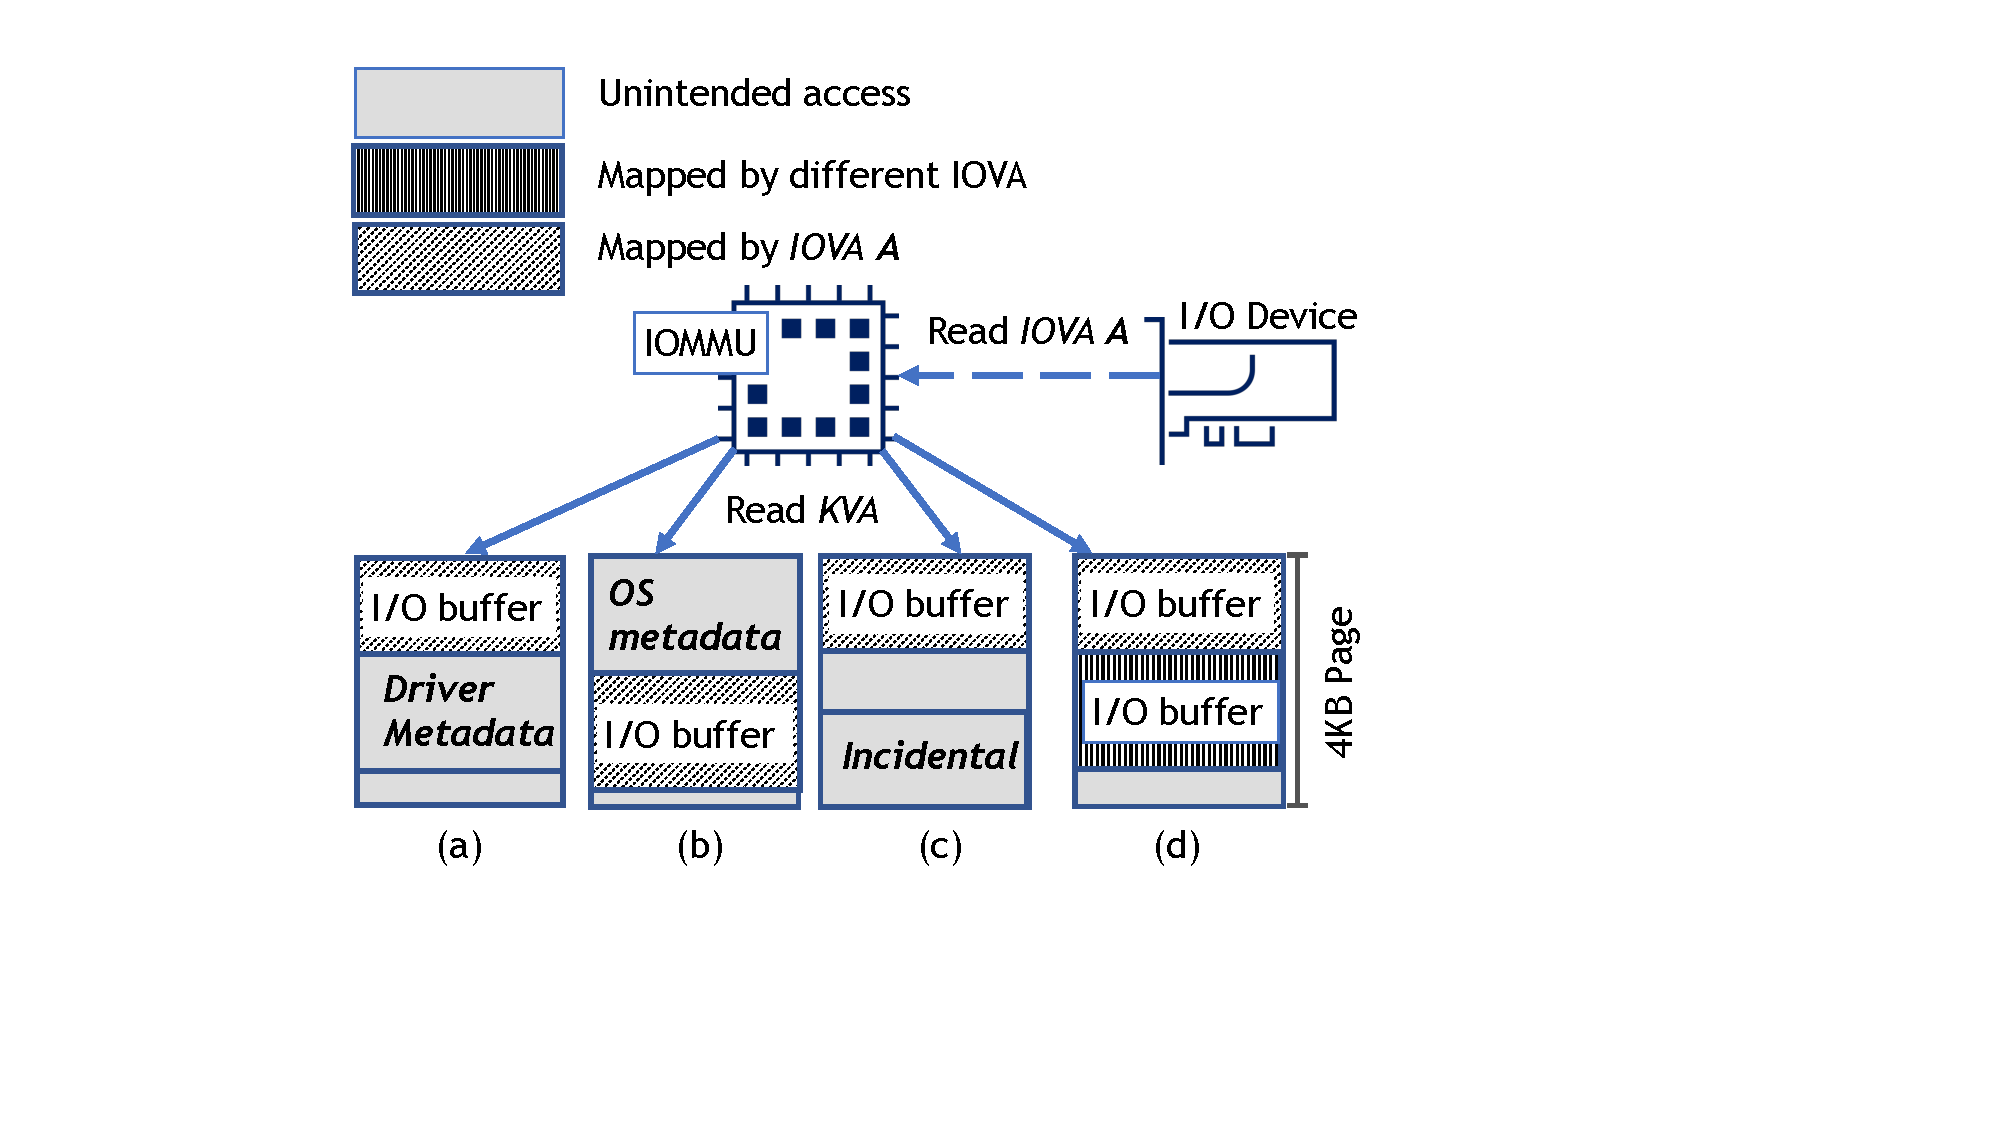
\includegraphics[width=0.9\columnwidth]{figs/subpage.pdf}
    \caption{\subpage{} DMA vulnerabilities when the I/O buffer shares a page with other data: (a) I/O buffer metadata; (b) OS
metadata; (c) a page mapped by multiple \iova; (d) randomly co-located sensitive buffers.}
    \label{fig:colocation}
\end{figure}

\subsection{Sub-Page Vulnerability}\label{sec:subpage}

We classify the different types of potentially co-located data, into four categories, as illustrated in Fig.~\ref{fig:colocation}:

\begin{enumerate}
    \item[(a)] The I/O buffer is part of a bigger data structure. In some cases, this data structure may include function pointers, often caused by poor DMA hygiene by the driver. We demonstrate a full exploit in Sec. \ref{sec:sbp2_attack}. An isolated driver fix is usually sufficient to fix such vulnerabilities.
    \item[(b)] The OS (e.g., memory allocator) rather than the driver saves metadata, such as free-lists, on the same page as the I/O buffer \cite{Cor07}. Manipulating these data structures may also compromise the system \cite{ak09}. Similarly to (a), sensitive metadata is unwittingly shared. However, in this case, it is an OS subsystem that is at fault rather than the device driver. We demonstrate attacks made possible by an OS subsystem in Sec. \ref{sec:linux_net}.
    \item[(c)] The same page is mapped multiple times due to co-located device driver buffers resulting in multiple \iova{} indicating the same page. A seemingly benign case, made dangerous by the fact that unmapping one \iova{} is meaningless, security-wise. The device will retain access to the physical page as long as a single valid \iova{} exists. We discuss the implications of this scenario in Sec. \ref{sec:linux_net}.
    \item[(d)] The I/O buffer and a different, dynamically allocated memory buffer may coincidentally share a page. This common situation results in data leakage (e.g., kernel pointers). Currently, the Linux kernel uses the same memory allocation mechanism (e.g., kmalloc) for both I/O buffers and regular kernel buffers. Consequently, I/O buffers often share pages with other, potentially sensitive, kernel buffers. Since IOMMU works in page granularity, the respective I/O devices gain access to these kernel buffers as well. This is a subclass of (b), as an OS subsystem causes it, but the main difference is that the exposed data structures are leaked randomly.

\end{enumerate}

In the next sections we demonstrate how a \simple{} attack utilizes type (a) vulnerability (Sec. \ref{sec:sbp2_attack}). A \emph{compound attack}, on the other hand, uses type (b) and (c) vulnerabilities (Sec. \ref{sec:linux_net}). 
We also demonstrate the risks associated with type (d) vulnerability in Sec. \ref{fig:dkasan-report}. Essentially, type (d) vulnerability simplifies KASLR subversion~(\ref{sec:kaslr}) and opens viable attack vectors. 


%KASLR is designed to stop code injection attacks. This indeed holds as long as kernel pointers are not leaked, an assumption that is not valid for DMA capable devices. For example, an OS leaks kernel pointers to a NIC, on pages containing small TX buffers. A malicious NIC can even spoof seemingly legitimate packets (e.g., ARP, ICMP, ICMPv6) to trigger kernel pointer leakage.

%Both attack types use type (d) vulnerability to compromise KASLR. KASLR is designed to stop code injection attacks. This indeed holds as long as kernel pointers are not leaked, an assumption that is not valid for DMA capable devices. For example, an OS leaks kernel pointers to a NIC, on pages containing small TX buffers. A malicious NIC can even spoof seemingly legitimate packets (e.g., ARP, ICMP, ICMPv6) to trigger kernel pointer leakage. \textcolor{olive}{We demonstrate the risks associated with type (d) vulnerability in Sec. \ref{fig:dkasan-report}.}

\begin{figure}[t]
    \centering
    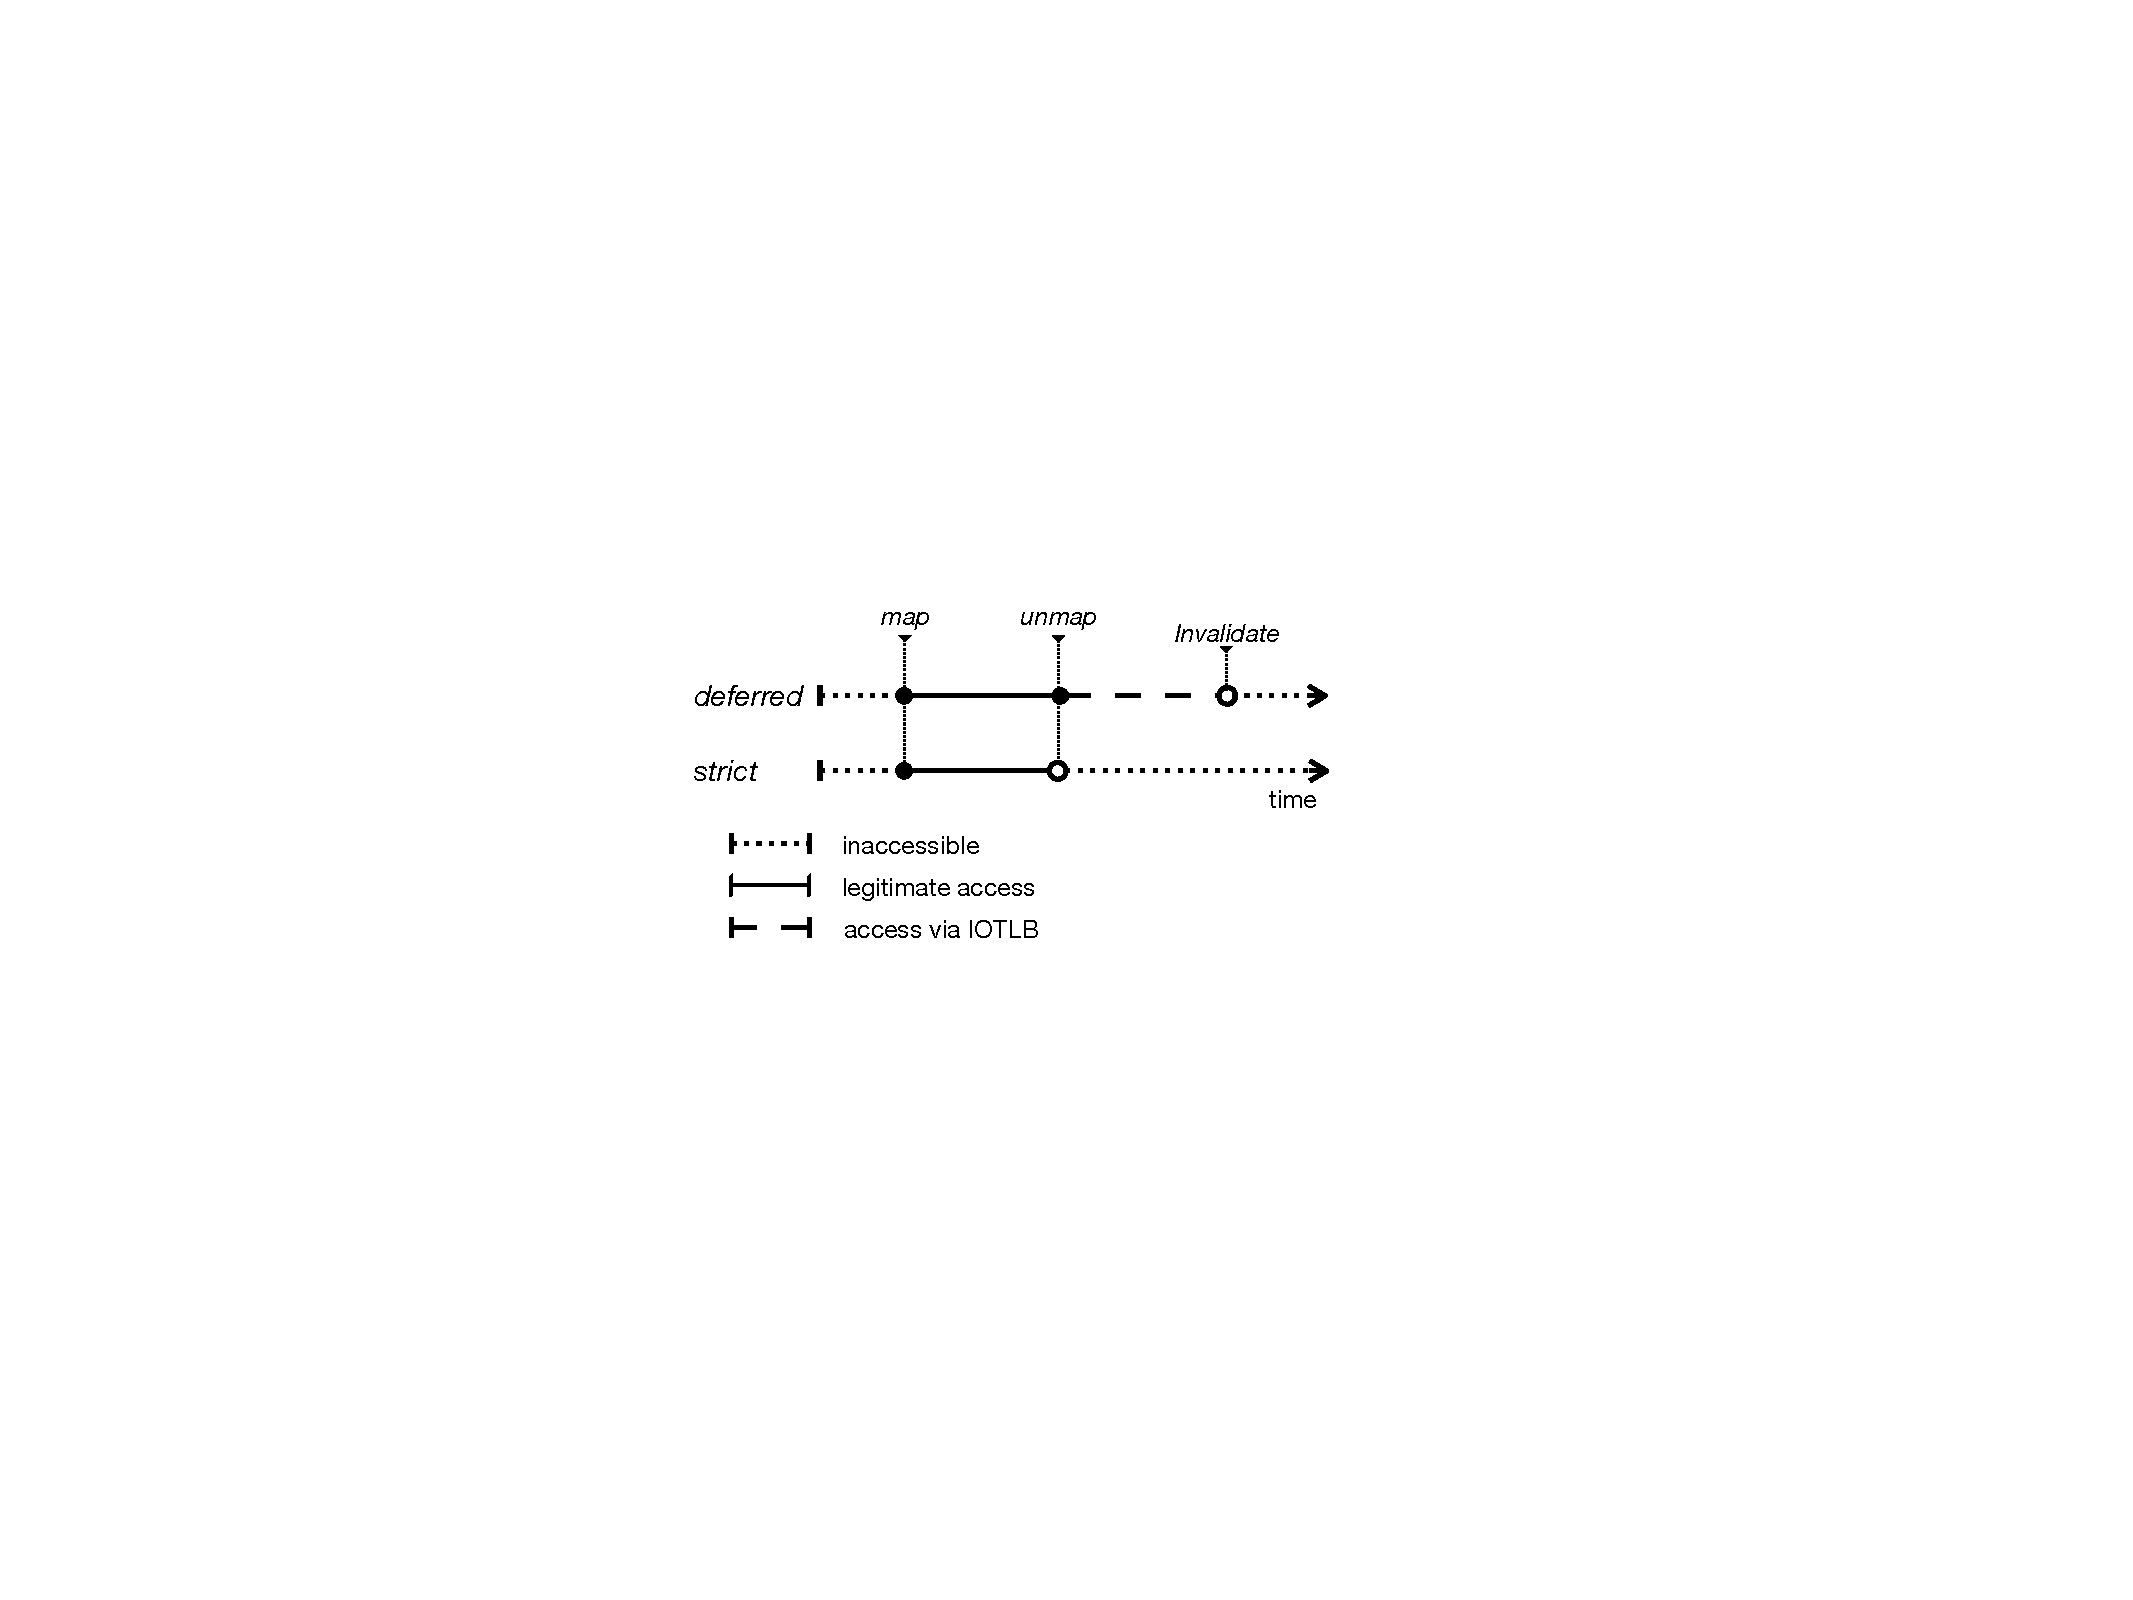
\includegraphics[width=0.9\columnwidth]{figs/strict.pdf}
    \caption{Strict vs. deferred IOTLB invalidation. In \emph{deferred} mode, there is a time window where the data is accessible to the device, but the mapping no longer appears in the page table.}
    \label{fig:deferred}
\end{figure}

\subsection{Deferred Invalidation vulnerability}\label{sec:deferred}

To limit the overhead of multiple memory accesses when translating \iova{} using page tables, the IOMMU caches translations in an I/O translation lookaside buffer (IOTLB). 

The IOTLB is analogous to the MMU TLB. IOMMU does not maintain consistency between the IOTLB and the IOMMU page tables. As a result, the OS has to explicitly invalidate the IOTLB to maintain consistency when a translation entry is removed. Namely, to ensure that the IOTLB never holds stale entries, the OS must invalidate the IOTLB immediately after it removes memory mappings. 

Yet, this scheme, called the \emph{strict} mode in Linux, can degrade performance, as IOTLB invalidations can induce very high overhead \cite{MMT16,MSMT18,Peleg15}. In I/O intensive workloads, the number of required IOTLB invalidations can be extremely high, as IOMMU entries are unmapped following each I/O operation. Moreover, the overhead of each IOTLB invalidation can be as high as 2000 cycles \cite{ABYTS11}. This is considerably higher than a TLB invalidation, which takes roughly 100 cycles \cite{Han14}. 

To reduce this overhead, Linux defers TLB invalidations by default and instead performs periodic global TLB invalidations. While \emph{deferred} mode, improves I/O performance, it also breaks the stipulation, that after unmapping (e.g., \texttt{dma\_unmap\_page}), the physical page should no longer be accessible by the device. This \emph{deferred} time frame (Fig. \ref{fig:deferred}), may be as high as 10 milliseconds \cite{MSMT18}.

The repercussions of \emph{deferred} mode are that a malicious device can take advantage of this time window, where it has access to memory pages, effectively, unbeknownst to the CPU. This opens up two distinct attack options:

\begin{enumerate}
    \item A device can alter data structures that the CPU has modified \emph{after} unmapping (e.g., calling \texttt{dma\_unmap\_page}).
    \iova{} mappings, as a rule, are short-lived as they should be used only for the duration of I/O, usually for a few microseconds. The additional milliseconds provide the attacker with a wide time-window sufficient to conduct her attack.
    \item The page can be freed, and then immediately reused by the OS. In fact, this is a common scenario, as Linux reuses \emph{hot} pages (i.e., recently used pages), as they are likely, to already reside in the CPU caches \cite{hotcold}. In turn, this opens up the kernel to additional random access attacks.
\end{enumerate}

%We demonstrate in Section \ref{sec:linux_net}, how an adversary can take advantage of \emph{deferred} mode.
\subsection{Threat Model}\label{sec:threat_model}

Our attacks are designed with the following assumptions:
\begin{enumerate}
    \item We assume the existence of a malicious DMA capable device attached to the system.
    \item The actual attack is performed solely by a DMA-capable malicious device.
    \item Any hardware aside from the specific malicious device is working as expected.
 \end{enumerate}

The most significant potential consequence of our attacks is privilege escalation, which allows attackers to execute arbitrary code with kernel privileges. Another potential consequence we consider is a full system memory dump. These are harder to thwart and even harder to detect. Lastly, a consequence of a possible failed attack is random memory corruption, resulting in a denial of service \cite{MMT16}, where the OS panics. Ideally, malformed devices should not be able to crash the entire system. 
